\documentclass{article}

%%%%%%%%PACKAGES%%%%%%%%
\usepackage{amsmath} 
\usepackage{mathtools}
\usepackage{amsfonts}
\usepackage{siunitx} 
\usepackage{physics}
\usepackage{geometry}
\usepackage{graphicx}
\usepackage{float}
\usepackage{hyperref}
\usepackage{url}
\geometry{margin=1in} 

%%%%%%%%TEOREMAS%%%%%%%%
\newtheorem{definition}{Definition}


%%%%%%%%COMANDOS%%%%%%%%
\newcommand{\pd}[2]{\frac{\partial #1}{\partial #2}}
\renewcommand{\L}{\mathcal{L}}

%%%%%%%%TITLE%%%%%%%%
\title{Notes on Higher-Form Symmetries}
\author{Gabriel C. Magalhães\footnote{gabriel.capelini@uel.br}}
\date{2026}

\begin{document}
\maketitle

\begin{abstract}
These notes present  my current understanding of higher-form symmetries and are intended for pedagogical purposes. They are continuously updated as I learn more about the subject and are based on the references listed in references section.
\end{abstract}

\tableofcontents
\pagebreak

\section{Introduction}
Higher-form symmetries generalize the conventional global symmetries by acting on extended operators, such as line or surface operators, rather than local, point-like ones. These ideas were considered first in \cite{Kapustin_2014}, but the foundational work was \cite{gaiotto_generalized_2015}. These symmetries are characterized by topological symmetry operators, and their action is defined via the linking between the manifold supporting the symmetry operator and the manifold supporting the charged operator. A key consequence is that the associated conserved currents become higher-degree differential forms, in contrast to the standard 1-form currents of ordinary symmetries.

To build intuition, we will first revisit the topological interpretation of ordinary symmetry operators before extending these ideas to the higher-form case. Here we follow the discussion of \cite{gomes_introduction_2023,bhardwaj_lectures_2024, tong_gauge_nodate,brennan_introduction_2023}.


\section{0-form symmetries}
One way to derive Noether's theorem was to make the parameter of the transformation, say, $\alpha$ local. That is, 
\begin{equation*}
	\alpha\to\alpha(x).
\end{equation*}
This led to 
\begin{equation}\label{0 form variation}
	\delta S=-\int d^4x\;\alpha(x)\partial_\mu j^\mu.
\end{equation}
Since $\alpha$ is arbitrary, if the equations of motion are satisfied, we have
\begin{equation}
	\partial_\mu j^\mu=0.
\end{equation} 
where $j^\mu$ is precisely the conserved current. Note that the conserved can be seen as a 1-form, and it has come from the symmetry parameter $\alpha$, which can be seen as a 0-form. Thefore, we now call the ``ordinary'' symmetries a \textit{0-form symmetry}, because the parameter of the transformation is a closed 0-form.

In terms of differential forms, the conservation law is written as
\begin{equation}
	d\star j=0,
\end{equation}
where $j$ is the current 1-form and $\star:\Lambda^p\to \Lambda^{D-p}$   is the Hodge star map that takes a $p$-form and associates it to a $(D-p)$-form. The conserved charges is given by
\begin{equation}
	Q\equiv\int d^{D-1}x\;j^0.
\end{equation}
In terms of differential forms, we write as
\begin{equation}
	Q=\int_{\Sigma_{D-1}}\star j,
\end{equation}
where $\Sigma_{D-1}$  is a $(D-1)$-dimensional manifold. Note that now the manifold in which the charge is defined is not necessarily a spatial manifold. We say then that those charges are integrated over a codimension-1 manifold, which is a submanifold of the $D$-dimensional manifold.  To understand how these operators act over the fields, we will make use of the \textit{Ward identity}\footnote{A deduction of the Ward identity can be found in \cite{schwartz_quantum_2014,gomes_introduction_2023}.},
\begin{equation}
	\partial_\mu\langle j^\mu(x)\phi(y)\rangle=-i\delta^{(D)}(x-y)\langle\delta\phi(y)\rangle.
\end{equation}
Integrating over a $D$-dimensional manifold $\Omega$  with boundary $\Sigma_{D-1}$, the left-hand side becomes
\begin{equation}
	\int_{\Omega}d\langle\star j\phi(y)\rangle=\int_{\Sigma_{D-1}}\langle\star j\phi(y)\rangle=\langle Q(\Sigma_{D-1})\phi(y)\rangle,
\end{equation}
where we have used Stokes theorem. For the right-hand side, we have
\begin{equation}
	-i\int_{\Omega}d^Dx\;\delta^{(D)}(x-y)\langle\delta\phi(y)\rangle,
\end{equation}
where we identify,
\begin{equation}
	\int_{\Omega}d^Dx\;\delta^{(D)}(x-y)=\begin{cases}0,\quad y\in\Omega\\1,\quad y\not\in\Omega\end{cases}
\end{equation}
as the \textit{linking} between the point $y$ and the manifold $\Omega$. Thus we call  
\begin{equation}
	\int_{\Omega}d^Dx\;\delta^{(D)}(x-y)\equiv \text{Link}(\Sigma_{D-1},y).
\end{equation}
Hence
\begin{equation}
	\langle Q(\Sigma_{D-1})\phi(y)\rangle=-i\text{Link}(\Sigma_{D-1},y)\langle\delta\phi(y)\rangle.
\end{equation}
What this expression is telling us, is that the charge acts on the local field, and it only have a non-vanishing action if the point where the local operator is defined lies within the manifold where the charge is defined. We can see that the link is invariant under a deformation on the manifold of the type $\Omega'=\Omega+\Omega_0$, with $\partial \Omega' = \Sigma',\partial \Omega = \Sigma$ and $y\not\in\Omega_0.$ Then 
\begin{equation}
	\langle Q(\Sigma + \partial\Omega_0)\phi(y)\rangle=\int_{\Omega\cup\Omega_0}\langle d\star j\phi(y)\rangle=\int_{\Omega}\langle d\star j\phi(y)\rangle+\int_{\Omega_0}\langle d\star j\phi(y)\rangle.
\end{equation}
Since $y\not\in\Omega_0$, then $\text{Link}(\Sigma_0,y)=0$, and
\begin{equation}
	\langle Q(\Sigma+\partial\Omega_0)\phi(y)\rangle=\int_{\Omega}\langle d\star j\phi(y)\rangle=\langle Q(\Sigma)\phi(y)\rangle.
\end{equation}
Thus, the computed charge will also be invariant. That is the reason why we call these operators \textit{topological}. The unitary operator is defined by taking the exponential of the conserved charge,
\begin{equation}
	U_g(\Sigma_{D-1})=\exp(i\alpha_aQ_a)=\exp\left(i\alpha\int\star j\right),
\end{equation}
where $g\in G$  is an element of some group $G$ and $\alpha_a$ are the parameters of the transformation. In the case of  $G=U(1)$,  we have $g=e^{i\alpha}$.  We say then that this is a topological codimension-1 operator. 

In terms of the unitary operator, the action over the local operators is given by
\begin{equation}
	\langle U_g(\Sigma_{D-1})\mathcal{O}(x)\rangle=\langle\mathcal{O}'(x)\rangle.
\end{equation}
We will use $\mathcal{O}(x)$ from now on to generalize the expressions to any local operator (not necessarily fields).  These expressions are evaluated inside correlators as a consequence of the Ward identity, but we can understand this in another way as well. Since the manifold where the topological operators are defined need not to be necessarily a spatial manifold, it does not make sense to compare two different operators at different times, since these are in different Hilbert spaces. But inside correlation functions, these operations are well-defined. To understand pictorially the action of topological operators, consider de figure below.

Let   $U(S^{D-1})$ be an operator defined over a $(D-1)$-sphere.  As we have seen, these operators act over local operators $\mathcal{O}(x)$ and transforms them into another operator $\mathcal{O}'(x)$  as shown in the figure
\begin{figure}[H]
	\centering
	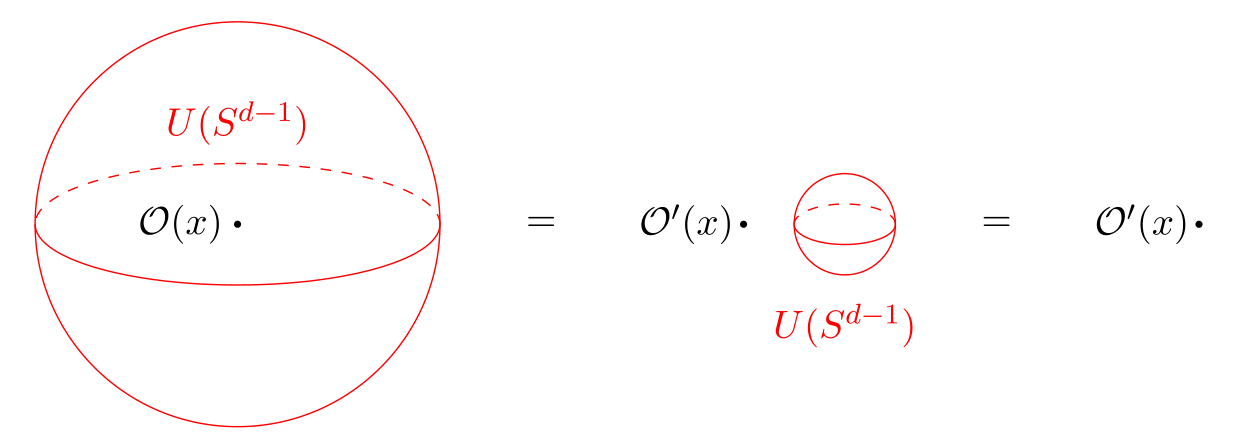
\includegraphics[scale=0.3]{figures/linking.png}
	\caption[The link of the $(D-1)$-sphere and the local operator $\mathcal{O}(x).$]{The link of the $(D-1)$-sphere and the local operator $\mathcal{O}(x).$ Taken from \cite{bhardwaj_lectures_2024}.}
\end{figure}
The operator $U(S^{D-1})$ has a non-trivial link with $\mathcal{O}(x)$. Note that it is impossible to remove the operator $\mathcal{O}(x)$ from the manifold $S^{D-1}$ without tearing it apart. Once we do this, we compute the action of the symmetry operator over the operator $\mathcal{O}$. Now $U(S^{D-1})$ is topologically equivalent to a point, thus we can deform it again and we are let only with the operator $\mathcal{O}'(x)$.   
\subsection{0-form Groups}
We define the 0-form group $G^{(0)}$ to be the group composed by the elements $g$ that parametrizes the operator $U_g.$

The composition of two topological operators is given by the composition law of the group,
\begin{equation}
	\langle U_g(\Sigma_{D-1})U_{g'}(\Sigma_{D-1})\rangle=\langle U_{gg'}(\Sigma_{D-1})\rangle.
\end{equation}
Thus, inserting the composition of topological operators into these correlation functions is equivalent to insert one topological operator with the composition of the elements. This is called the fusion rule,
\begin{equation}
	U_g\otimes U_{g'}=U_{gg'}.
\end{equation}
Therefore, the local operators transform under representations of the 0-form group $\mathcal{R}(g)$, 
\begin{equation}
	\langle U_g(\Sigma_{D-1})\mathcal{O}(x)\rangle=\mathcal{R}(g)\langle\mathcal{O}(x)\rangle.
\end{equation}
From now on, we will drop the correlation function notation, but it is there unless it said the contrary. 

\section{$p$-form Symmetries}
$p$-form symmetries are straightforward generalization of 0-form symmetries. The parameter of the transformation is a $p$-form and the associated currents will be $(p+1)$-forms. Therefore, the symmetry operators associated to these symmetries will be codimension-$(p+1)$ operators. 


To see why it must be a codimension-$(p+1)$ operator, we go back to Eq.(\ref{0 form variation}). For a $D$-dimensional space and in the language of differential forms, this equation becomes 
\begin{equation}
	\delta S=\int\star j\wedge d\alpha.
\end{equation}
Now $\alpha$  is a $p$-form, consequently $d\alpha$ will be a $(p+1)$-form. Then, in order to match the dimension of the spacetime, $\star j$ must be a $(D-p-1)$-form. This implies that the conserved charge will be 
\begin{equation}
	Q=\int_{\Sigma_{D-p-1}} \star j,
\end{equation}
and the unitary operator is defined as before
\begin{equation}
	U_g(\Sigma_{D-p-1})=\exp\left(i\alpha\int_{\Sigma_{D-p-1}}\star j\right),
\end{equation}
where now this is understood as a codimension-($p+1$) operator. There is one subtletie about the parameter $\alpha$. One may question why the parameter $\alpha$ that parametrizes the unitary operator is a number, it should not be a $p$-form? The answer is that these are the components of the $p$-form. Therefore, for each component, we have a different unitary operator. This expression is just written a concise and general manner.

The group of $p$-form symmetries $G^{(p)}$  consists of the elements that parametrize the operator $U_g(\Sigma_{D-p-1}).$ Just as before, the composition of those operators is given by  
\begin{equation}
	U_g(\Sigma_{D-p-1})U_{g'}(\Sigma_{D-p-1})=U_{gg'}(\Sigma_{D-p-1}).
\end{equation}
Moreover, the $p$-form symmetry group is abelian for $p\ge 1.$ This follows because we can deform an operator over another without ever crossing them, as shown in figure (\ref{fig:commutationextendedoperators}). We now must look at which objects are charged under those symmetries, that is, which objects the $p$-form operators act on. 

\begin{figure}
	\centering
	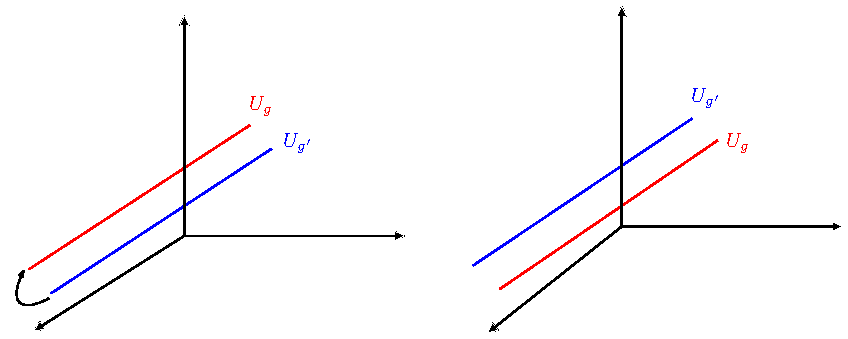
\includegraphics[width=1.\linewidth]{figures/interchanging_topological_operators.pdf}
	\caption{The operators $U_g$ and $U_{g'}$ defined on spacetime may have their ordering interchanged without one crossing another.}
	\label{fig:commutationextendedoperators}
\end{figure}


\subsection{Action of $p$-form symmetries}
The 0-form symmetries act over local operators, which are supported on 0-dimensional regions. We say then that the local operators are \textit{charged} under the 0-form symmetry. We now wish to understand which objects are charged under $p$-form symmetries. It is straightforward to note that for $p\geq1,$ the $p$-form symmetry will never act over a local operator because we can always deform the operator in a way that it does not link with the point. Therefore, the $p$-form symmetry acts over objects that have a dimension $q\geq p$.

\subsection*{Case $q=p$}
We define an operator $U_g(\Sigma_{D-p-1})$ over a $(D-p-1)$-dimensional manifold that links with some operator  $\mathcal{O}(M_p)$ defined over a $p$-dimensional manifold. Then we deform $U_g(\Sigma_{D-p-1})$  over $\mathcal{O}(M_p)$, leaving behind a phase $\phi(g)$ in which,  
$$
\phi(g)\in \mathbb{C}^{\times},\quad \mathbb{C}^{\times}\equiv \mathbb{C}\backslash\{\ \!\!0 \}.
$$
The action of the operator $U_g(\Sigma_{D-p-1})$ over $\mathcal{O}(M_p)$ is represented below. 
\begin{figure}[H]
	\centering
	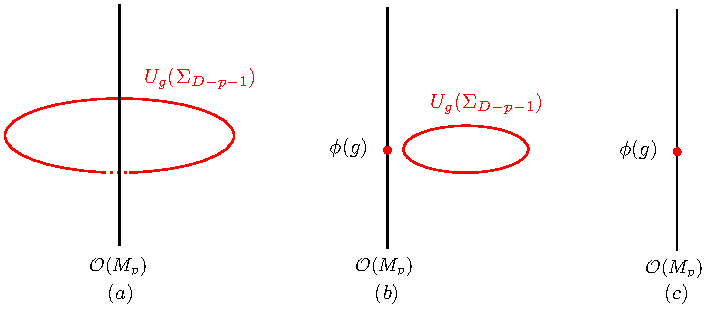
\includegraphics[scale=1]{figures/linking2.pdf}
	\caption[Link of extended operators.]{Link between extended operators. In $(a)$ the topological operator $U_g(\Sigma_{D-p-1})$ and the extended operator $\mathcal{O}(M_p)$ have a non-trivial link. In $(b)$, $U_g(\Sigma_{D-p-1})$ is deformed and passes trough $\mathcal{O}(M_p)$ leaving behind a phase $\phi(g)$. In $(c)$, $U_g(\Sigma_{D-p-1})$ and $\mathcal{O}(M_p)$ no longer have a link, then  $U_g(\Sigma_{D-p-1})$ is deformed to a point.} 
\end{figure}
\noindent The action of the topological extendend operators are given in terms of the Ward identity, 
\begin{equation}
	U_g(\Sigma_{D-p-1})\mathcal{O}(M_p) = e^{iq\lambda\text{Link}(\Sigma,M)}\mathcal{O}(M_p)U_g(\Sigma'_{D-p-1}),
\end{equation}
where $\Sigma'_{D-p-1}$ is a manifold homotopic to $\Sigma_{D-p-1}$ which does not link with $M_p$. The composition of the group induces a composition of those functions $\phi(g)$, 
\begin{equation}
	\phi(g)\phi(g')=\phi(gg').
\end{equation}
Therefore the functions $\phi(g)$ form a 1-dimensional representation of the $p$-form group $G^{(p)}$.  Since $G^{(p)}$ is an abelian group, from Schur’s Lemma we know that every irreducible representation of this group is 1-dimensional. Hence the functions $\phi(g)$ form precisely the irreducible representation of the group $G^{(p)}$. Therefore, the operators $\mathcal{O}(M_p)$ transforms under the fundamental representations of the $p$-form group, which shows that the charged objects under $p$-form symmetries are extended operators supported on $p$-dimensional manifolds. The case $q>p$ are out of the scope of this work. A discussion on the subject can be found in some references such as \cite{Bhardwaj_2024,bartsch2023higherrepresentationsextendedoperators}. 

\subsubsection{Higher-form symmetries in $D-$dimensional $U(1)$ gauge theory.}
Let $A$ be a 1-form $U(1)$ gauge field with 
\begin{equation}\label{conservation law maxwell}
	F=dA,
\end{equation}
where $F$ is a 2-form. In $D=4$ this is exactly Maxwell theory. From (\ref{conservation law maxwell}) we have
\begin{equation}\label{conservation F}
	dF=d\star(\star F)=0. 
\end{equation}
Therefore the Noether current then is the $(D-2)$-form (up to normalizations)
\begin{equation}
	J^m = \frac{1}{2\pi}\star F.
\end{equation}
The conserved charge is 
\begin{equation}
	Q^m=\frac{1}{2\pi}\int_{\Sigma_2}\star (\star F)=\frac{1}{2\pi}\int_{\Sigma_2}F,
\end{equation}
and the unitary operator is 
\begin{equation}
	U_g^m(\Sigma_2)=\exp\left(\frac{\alpha_m}{2\pi}\int_{\Sigma_2}F\right).
\end{equation}
The index $m$ stands for \textit{magnetic symmetry}. Below we will explain the reason for this name. For $p\geq 1$-forms we integrate the charge over a $(D-p-1)$ manifold. Since this is 2-dimensional manifold, $D-p-1=2\Rightarrow p=D-3$. Thus, the magnetic symmetry is related to a $(D-3)$-form. 

The other conservation law follows from the vacuum Maxwell equations,
\begin{equation}\label{conservation F star}
	d\star F=0,
\end{equation} 
which implies that in this case the conserved current is the 2-form,
\begin{equation}
	J^e = \frac{1}{e^2}F.
\end{equation}
The conserved charge is 
\begin{equation}
	Q^e=\frac{1}{e^2}\int_{\Sigma_{D-2}}\star F, 
\end{equation}
And the unitary operator
\begin{equation}
	U^e_g(\Sigma_{D-2})=\exp\left(\frac{i\alpha_e}{e^2}\int_{\Sigma_{D-2}}\star F\right).
\end{equation}
This is the \textit{electric symmetry}. In this case, $D-p-1=D-2\Rightarrow p=1$. Then, the electric symmetry is a 1-form symmetry, independent of the dimension. 

Therefore, this $U(1)$ gauge theory has two higher-form symmetries, an \textit{electric 1-form symmetry} and a \textit{magnetic ($D-3$)-form symmetry.} We represent the symmetry group as 
\begin{equation}
	U(1)^1_e\times U(1)^{D-3}_m. 
\end{equation}
For the case $D=4$, the charged objects under the electric 1-form symmetry are the \textit{Wilson lines $W_{q_e}(L)$},
\begin{equation}
	W_{q_e}(L)\equiv\exp\left(iq_e\int A\right),
\end{equation}
where $q_e$ is the charge of the Wilson line. The Wilson line is interpreted as the worldline of a probe particle with electric charge $q_e$.

Written explicitly in components 
\begin{equation}
	W_{q_e}(L)=\exp\left(iq_e\oint dx^\mu A_\mu\right)=\exp\left(iq_e\oint dx^0A_0+iq_e\oint dx^iA_i\right).
\end{equation}
Note that if we perform a large gauge transformation in $a_0$,
\begin{equation}
	A_0\to A_0+\partial_0\Lambda, \quad \Lambda =\frac{2\pi}{L_0}x^0,
\end{equation} 
we see that, for the zeroth component of the Wilson line, 
\begin{equation}
	\exp\left(iq_e\oint dx^0A_0\right)\exp\left(iq_e\oint dx^0 \frac{2\pi}{L_0}\right)=\exp\left(iq_e\oint dx^0 a_0\right)\exp(2\pi i q_e). 
\end{equation} 
Hence, in order to the Wilson line to be gauge invariant, we must have $q_e\in \mathbb{Z}.$ 

From Maxwell action, one can compute the canonical momentum associated do the dynamical gauge field. It will be exactly $J^e$. This implies that the action of the electric 1-form symmetry on the gauge fields is a shift by a flat connection 
\begin{equation}
	A \to A + \alpha_e.
\end{equation}
Consequently, its action on the Wilson lines will be 
\begin{equation}
	U_g^e(\Sigma_{D-2})W_{q_e}(L) = e^{iq_e\alpha_e}W_{q_e}(L)U_g^e(\Sigma_{D-2}'),
\end{equation}
where $\Sigma_{D-2}'$ is homotopic to $\Sigma_{D-2}$ and does not link with $L$. 

The magnetic $(D-3)$-form symmetry acts on 't Hooft lines, which is interpreted the wordline of a probe particle with magnetic charge $q_m$. To write explictly the 't Hooft line, we introduce dual field $\hat{A}$ following from Eq.(\ref{conservation F star}),
\begin{equation}
	\star F = d\hat{A}.
\end{equation}
Thus, we define the 't Hooft line as 
\begin{equation}
	T(L) \equiv \exp\left(iq_m\int \hat{A}\right).
\end{equation}
Analogously to the electric 1-form symmetry, the magnetic $(D-3)$-form symmetry acts by shifting the dual field $\hat{A}$ by flat connections,
\begin{equation}
	\hat{A} \to \hat{A} + \alpha_m.
\end{equation}
Consequently, the action on 't Hooft lines will give 
\begin{equation}
	U_g^m(\Sigma_2)T(L) = e^{iq_m\alpha_m}T(L)U_g^m(\Sigma_2'),
\end{equation}
where $\Sigma_2'$ is homotopic to $\Sigma_2$ and does not link with $L$. 
\subsubsection{Higher-form symmetries in Chern-Simons theory}
We will now discuss how higher-forms arise in Chern-Simons theory and how do we extract crucial information of this theory using this framework.

Consider Chern-Simons action, 
\begin{equation*}
	S_{CS}=\int d^3x \frac{k}{4\pi}\epsilon_{\mu\nu\rho}a_\mu\partial_\nu a_\rho.
\end{equation*}
We can take the commutation relations from it. Choosing the gauge $a_0=0$, we get 
\begin{equation}
	S_{CS}=\int d^3x\frac{k}{4\pi}\epsilon^{ij}a_i \dot{a}_j.
\end{equation}
The canonical momenta will be 
\begin{equation}
	\Pi_j=\pd{\L}{\dot{a}_j}=\frac{k}{4\pi}\epsilon_{ij}a_i.
\end{equation}
Imposing the commutation relation 
\begin{equation}
	\comm{a_i(x)}{\Pi_j(y)}=i\delta_{ij}\delta(x-y), 
\end{equation}
we have
\begin{equation}
	\begin{split}
		&\comm{a_i(x)}{\frac{k}{4\pi}\epsilon_{kj}a_k(y)}=i\delta_{ij}\delta(x-y).
	\end{split}
\end{equation}
Multiplying by $\epsilon^{jm}$ on both sides, 
\begin{equation}
	\comm{a_i}{a_m}=\frac{4\pi i}{k}\epsilon_{im}\delta(x-y). 
\end{equation}
This implies 
\begin{equation}
	\comm{a_1(x)}{a_2(y)}=\frac{4\pi i}{k}\delta(x-y).
\end{equation}
That is, the components of the gauge field do not commute with each other. We construct the Wilson lines of the theory, 
\begin{align}
	&W^1(C_1)\equiv\exp\left(iq\oint_{C_1}dx^1 a_1\right),\\
	&W^2(C_2)\equiv\exp\left(iq\oint_{C_2}dx^2 a_2\right),
\end{align}
and compute $W^1W^2$. Using BCH formula 
\begin{equation}
	W^1W^2=\exp\left(i\oint_{C_1}dx a_1+i\oint_{C_2}dy a_2+\frac{1}{2}dxdy\comm{a_1}{a_2}\right)=W^2W^1\exp\left(\frac{2\pi i}{k}\oint dxdy\delta^2(x-y)\right).
\end{equation}
where we considered $q=1$ for simplicity. Therefore, 
\begin{equation}\label{wilson lines commutation}
	W^1W^2=e^{-\frac{2\pi i}{k}}W^2W^1.
\end{equation}
We may also compute the conserved quantities. Writing the Chern-Simons action in terms of differential forms,
\begin{equation}
	S_{CS}=\int \frac{k}{4\pi}a\wedge da, 
\end{equation}
we see from the equations of motion for $a$ that, 
\begin{equation}
	da=0. 
\end{equation}
This is precisely the conservation law for a 1-form symmetry. The conserved charge then is,
\begin{equation}
	Q(C)=q\oint_C a.
\end{equation}
form some curve $C$ and parameter $q$. The unitary operator is 
\begin{equation}\label{wilson line cs}
	W(C)=\exp\left(iq\oint_C a\right).
\end{equation}
It is now clear that this is a Wilson line in the Chern-Simons theory and $q$ is its charge. Using the same method that we used for the Wilson lines in Maxwell theory, one can show that $q\in\mathbb{Z}$. We may label the Wilson lines by an integer that represents its charge, e.g., $W_n(C)$. 

From (\ref{wilson lines commutation}) we see that the Wilson lines act over another  Wilson line. However, from (\ref{wilson line cs}) we see that the Wilson lines are symmetry operators as well. Thus, the Wilson lines in Chern-Simons theory are the charged objects and the symmetry operators at the same time. Since these are symmetries, 
\begin{equation}
	\comm{H}{W}=0. 
\end{equation}
Therefore the energy eigenstates are also eigenstates of $W^1$ and $W^2$, but it cannot be the same eigenstate for both, since $W^1$ and $W^2$ do not commute with each other. This reveals that our theory has a degeneracy. To see the order of the degeneracy, apply an energy eigenstate $|n\rangle$ in (\ref{wilson lines commutation}), 
\begin{equation}\label{non commutation wilson lines}
	W^1W^2|n\rangle=e^{-\frac{2\pi i}{k}}W^2W^1|n\rangle=\omega_1e^{-\frac{2\pi i}{k}}W^2|n\rangle, 
\end{equation}
where $\omega_1$ is the eigenvalue of $W^1$. Now apply $W^2$ $k$ times in this equation. We can use the commutation relation to change the order of the operators. Each time we do this, we get a phase $e^{-\frac{2\pi i}{k}}$, obtaining 
\begin{equation}
	W^1(W^2)^k|n\rangle=\omega_1(W^2)^k|n\rangle.
\end{equation}
This shows that after $k$ applications, $W^2$ becomes an eigenstate of $W^1$ and therefore we no longer have a degeneracy. This shows that this degeneracy is of order k. 
More generally, applying $W^1$ $n$ times and $W^2$ $m$ times, we get
\begin{equation}
	(W^1)^n(W^2)^m=e^{-\frac{2\pi i}{k}nm}(W^2)^m(W^1)^n,\;m,n\in\mathbb{Z}.
\end{equation}
Then $(W^1)^k$ or $(W^2)^k$ behave as the identity. Then it appears that the lines $n$ and $n+k$ can be identified. However this  identification is not straightforward. Too see this, consider the link between two Wilson lines, where one line extends to the infinity and the other is closed around this first line, as represented in the Fig.(\ref{fig:wilsonlineslink}),
\begin{figure}[h]
	\centering
	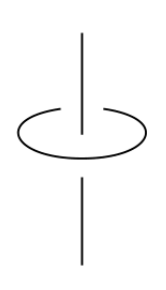
\includegraphics[width=0.2\linewidth]{figures/wilson_lines_link}
	\caption[Link between two Wilson lines.]{Link between two Wilson lines. Taken from \cite{gomes_introduction_2023}.}
	\label{fig:wilsonlineslink}
\end{figure}

We can think of these lines as the wordlines of some particle with statistics $\nu$ and spin $s=\nu/2$. The statistics is computed by looking at the phase $e^{\pm i\nu\pi}$ that the particles acquire upon the exchange. This is equivalent to perform half of a turn and then translate the particle. Then, from (\ref{wilson lines commutation}),
\begin{equation}
	W_n(C)W_n(C')=e^{-\frac{2\pi in^2}{k}}W_n(C')W_n(C).
\end{equation} 
Wich shows that 
\begin{equation}
	\nu=\frac{n^2}{k}\;\text{mod }2\Rightarrow s=\frac{n^2}{2k}\;\text{mod }1.
\end{equation}
Therefore, a line with $n+k$ have a statistics, 
\begin{equation}
	v=\frac{n^2}{2}+2n+k.
\end{equation}
This lead to two conclusions. 

\begin{itemize}
	\item \textbf{for even k:} we may parametrize $k$ as $k=2m,m\in\mathbb{Z}$. Since $\nu$ is defined mod 2, then $\nu(n)$ and $\nu(n+k)$ are identified and therefore there are $k$ independent lines. 
	\item \textbf{for odd k:} we may parametrize $k$ as $k=2m+1,m\in\mathbb{Z}$. Then $\nu(n)$ and $\nu(n+k)$ differ mod 1 and to identify the lines we must take $k\to 2k$. Therefore, there are 2k independent lines. 
\end{itemize}
\subsection{Spontaneous symmetry breaking of higher-form symmetries}
At the end of the day, we are working with symmetries. Therefore we can use the framework we are used to and apply to higher-form symmetries as well. One interesting feature that symmetries exhibit is that it can be spontaneously broken. 

Recall the definition of SSB. To know whether or not a symmetry is spontaneously broken, we evaluate the expectation value of a operator $\mathcal{O}(x)$ that is charged under the symmetry. Then we concluded that
\begin{equation}\label{ssb definition 5}
	\langle \mathcal{O}(x)\rangle
	\begin{cases}
		= 0,\quad \text{symmetric phase,}\\
		\neq 0,\quad \text{symmetry broken phase. }
	\end{cases}
\end{equation}

For $p$-form symmetries, this behavior can be translated as follows. The charged operators are $p$-dimensional operators. In general, the expectation value of such operators can be written as, 
\begin{equation}
	\langle \mathcal{O}(\Sigma_p)\rangle \sim e^{-f(\Sigma_p)},
\end{equation}
where $f(\Sigma_p)$ is an arbitrary function. Define the function $\text{Vol}(\Sigma_p)$. Note that this function does not compute the volume enclosed by $\Sigma_p$ but the appropriate dimension. For example, for $p=1$, the ``volume'' is the perimeter of the curve $\Sigma_p$. Therefore, we may reproduce the behavior of Eq.(\ref{ssb definition 5}) as
\begin{equation}
	\lim_{\text{Vol}(\Sigma_p)\to\infty}\left(\frac{f(\Sigma_p)}{\text{Vol}(\Sigma_p)}\right)=\begin{cases}
		\infty,\quad\text{symmetric phase},\\
		\text{finite},\quad\text{{symmetry broken phase}}.
	\end{cases}
\end{equation}
Note that for the finite case, we can always add a counter-term and define a renormalized operator,
\begin{equation}
	\hat{\mathcal{O}}(\Sigma_p) \equiv \exp\left(-c\oint_{\Sigma_p}dV \right)\mathcal{O}(\Sigma_p),
\end{equation}
such that 
\begin{equation}
	\langle \hat{\mathcal{O}}\rangle \neq 0. 
\end{equation}
Therefore, the vacuum is charged under the generalized symmetry. For the infinite case, there is no way we can surpass this behavior by adding a local counter-term and the vacuum is not charged under the generalized symmetry. These ideas are rather abstract, but now we will give an example where we will use objects that we are used to. 
\subsubsection{Spontaneous symmetry breaking in Maxwell theory}
As we have seen, the charged operators in Maxwell theory are the Wilson and 't Hooft lines. The Wilson loop is known for having a expectation value depending on geometrical properties, such as the area enclosed by the curve $C$ where it is defined or the perimeter of the curve, 
\begin{align}
	&\langle W(C) \rangle \sim e^{-\text{Area}(C)},\\
	&\langle W(C) \rangle \sim e^{-\text{Perimeter(C)}}. 
\end{align}
The area decays faster than the perimeter of the curve, 
\begin{align}
	&	\lim_{\text{Perimeter}(C)\to\infty}\left(\frac{\text{Area}(C)}{\text{Perimeter}(C)}\right) \to \infty, \\
	& \lim_{\text{Perimeter}(C)\to\infty}\left(\frac{\text{Perimeter}(C)}{\text{Perimeter}(C)}\right) \to \text{finite.}
\end{align}
In this case, Vol($\Sigma_p$) is a the perimeter of the curve $C$. 
Essentially, what we have is that
\begin{align}
	&e^{-\text{Area}(C)} \to 0\\
	&e^{-\text{Perimeter(C)}} \neq 0.
\end{align}
Therefore, the Wilson loop is a good choice for an order parameter for the SSB in Maxwell theory. We now proceed to do this for a 1-form symmetry and show a very exciting result.  

We have shown that a Goldstone boson can be understood as the amplitude 
\begin{equation}
	\langle n,\vec{k}| j_{\mu\nu}|0\rangle,
\end{equation}
where $n$ is some quantum number (in our deduction was the energy) and $\vec{k}$ its momentum. We will compute this amplitude considering the one-photon state $|\lambda,\vec{k}\rangle$ with polarization $\lambda$ and momentum $\vec{k}$. The one photon state is given by the action of the creation operator for photons on the vacuum, 
\begin{equation}
	|\lambda,\vec{k}\rangle=A_\lambda^{\dagger}(k)|0\rangle,
\end{equation}
When quantizing Maxwell theory, we note that the Lorentz gauge $\partial_\mu A^{\mu}$ does not hold as a operator equation since this would lead to contradictions in the commutation relations. We must impose this as a equality acting on physical states, that is, 
\begin{equation}
	\partial_\mu A^{\mu}|\text{phys}\rangle =0.
\end{equation}
This implies that there are some degrees of freedom that are not physical. These discussions presented here were brief but are quite standard and can be found in many QFT books

Suppose that only $\lambda=1,2$ are the physical ones. The gauge field can be written as 
\begin{equation}
	A^{\mu}(x)=\frac{1}{(2\pi)^{3/2}}\int \frac{d^3\vec{p}}{2|\vec{p}|}\sum_{\lambda=1}^2e^{\mu}_{\;\;\lambda}(p)(A_\lambda(p)e^{-pix}+A_\lambda(p)e^{ipx}).
\end{equation}
The commutation relations are
\begin{equation}
	\comm{A_\lambda(p)}{A^{\dagger}_{\lambda'}(p')}=2|\vec{p}|\delta_{\lambda,\lambda'}\delta^3(\vec{p}+\vec{p}')
\end{equation}
Now we compute 
\begin{equation}
	\langle 0|F_{\mu\nu}|\lambda,\vec{p}\rangle=\langle 0|(\partial_\mu A_\nu-\partial_\nu A_\mu)A_\lambda^{\dagger}(p)|0\rangle.
\end{equation}
One of the terms is 
\begin{equation}
	\partial_\mu A_{\nu}=\frac{i}{(2\pi)^{3/2}}\frac{d^3p}{2|\vec{p}|}\sum_{\lambda=1}^2p_\mu\epsilon_{\nu}^{\;\;\lambda}(A_\lambda^{\dagger}(p)e^{ipx}-A_{\lambda}(p)e^{-ipx})
\end{equation}
Thus, 
\begin{equation}
	\langle 0|\partial_{\mu}A_\nu A_\lambda^\dagger|0\rangle = \frac{i}{(2\pi)^{3/2}}\langle 0|\int\frac{d^3p'}{|\vec{p}'|}\sum_{\lambda'=1}^{2}\epsilon_\nu^{\;\;\lambda'}(A_{\lambda'}^{\dagger}(p')e^{ip'x'}-A_{\lambda'}e^{ip'x'})A_\lambda^{\dagger}(p)|0\rangle.
\end{equation}
Using the commutation relations, we get 
\begin{equation}
	\begin{split}
		\langle 0|\partial_{\mu}A_\nu A_\lambda^\dagger|0\rangle &= \frac{i}{(2\pi)^{3/2}}\langle 0|\int \frac{d^3p'}{2|\vec{p}'|}\sum_{\lambda'=1}p'_\mu\epsilon_\nu^{\;\;\lambda'}A_{\lambda'}^{\dagger}(p')A_\lambda^{\dagger}(p)e^{ipx}|0\rangle\\&
		-\frac{i}{(2\pi)}e^{-px}\langle 0|\epsilon_\nu^{\;\;\lambda}p_\mu|0\rangle = \frac{i}{(2\pi)^{3/2}}e^{-ipx}\epsilon_\nu^{\;\;\lambda}p_\mu,
	\end{split}
\end{equation}
where the first term vanishes as the creation operators acts on the vacuum at its left. The order term gives the same contribution but with the indices exchanged. Thus 
\begin{equation}
	\langle 0| F_{\mu\nu}|\lambda, \vec{p}\rangle = \frac{i}{(2\pi)^{3/2}}e^{-ipx}(\epsilon_\mu^{\;\;\lambda}p_\nu-\epsilon_\nu^{\;\;\lambda}p_\mu).
\end{equation}
This shows that the photon is the Goldstone boson arising from the spontaneous symmetry breaking of a 1-form symmetry in Maxwell theory. 

There are fair questions to be asked. Which symmetry is being broken here? Since Maxwell theory possesses two 1-form symmetries, would we get two Goldstone bosons? 

There is an expression that relates the number of Goldstone bosons $n_{GB}$ to the number of broken symmetry generators $n_{BS}$ \cite{Watanabe_2011}, 
\begin{equation}
	n_{GB} - n_{BS} = \frac{1}{2}\text{rank}(\rho)
\end{equation}
where 
\begin{equation}
	i\rho_{ab} \equiv \lim_{\Omega\to\infty}\frac{1}{\Omega}\langle 0|[Q_a,Q_b]|0\rangle. 
\end{equation}
The charged operators, that is, the Wilson and 't Hooft lines, do not commute. In fact, 
\begin{equation}
	\comm{W(C)}{T(C')} \sim \text{Link}(W,T). 
\end{equation}
Therefore, the photon arises due to some complicated mixture of both symmetries.

Note that if we add electric matter, Eq.(\ref{conservation F star}) is no longer a symmetry. Nevertheless, a Goldstone boson (the photon) still arises due to Eq.(\ref{conservation F}). Conversely, if we add magnetic matter, Eq.(\ref{conservation F}) ceases to be a symmetry, while Eq.(\ref{conservation F star}) remains intact. Therefore, unless both conservation laws are explicitly broken, the photon always appears as a Goldstone boson.
\section{Discrete Gauge Theory}
Discrete gauge transformations belong to discrete groups, rather continuous ones. It can be better understood in terms of higher-form symmetries. Before we understand how this works, we need to introduce two concepts, the \textit{Pontryagin dual} and the \textit{Screening} of operators. 
\subsection{Pontryagin Dual}
For some $p$-form symmetry group $G^{(p)}$ we may define the homomorphisms
\begin{equation}
	\phi:G^{(p)}\to U(1). 
\end{equation}
These maps form a group with the composition given by
\begin{equation}
	\phi(g)\phi'(g)=(\phi\phi')(g)\in U(1).
\end{equation}
We denote this group by 
\begin{equation}
	\widehat{G}^{(p)}=\{\text{all homomorphisms }G^{(p)}\to U(1) \}.
\end{equation}
Let us ilustrate this idea with two examples. 
\subsubsection*{Example: $G^{(p)}=U(1)$}
\noindent Define the homomorphism as,
\begin{equation}
	\phi(g)=g^q=e^{i\alpha q},\; \alpha\in [0,2\pi),\;q\in\mathbb{Z}.
\end{equation}
Let 
\begin{align}
	&\phi_1(g)=g,\\
	&\phi_2(g)=g^2\\
	&\phi_3(g)=g^3.
\end{align}
The composition gives, 
\begin{equation}
	\phi_1(g)\phi_2(g)=\phi_3(g). 
\end{equation}
This is the composition rule of the $\mathbb{Z}$ group. Therefore the Pontryagin dual for $U(1)$ is 
\begin{equation}
	\widehat{G}^{(p)}=\mathbb{Z}.
\end{equation}
\subsubsection*{Example: $G^{(p)}=\mathbb{Z}_N$}
In this case, $g=e^{\frac{2\pi i\alpha}{N}}$. Defining the homomorphism as 
\begin{equation}
	\phi=g^q=e^{\frac{2\pi i\alpha q}{N}}.
\end{equation}
Take $N=3$ and let 
\begin{align}
	&\phi_1(g)=g,\\
	&\phi_2(g)=g^2. 
\end{align}
The composition gives 
\begin{equation}
	\phi_1(g)\phi_2(g)=\phi_1(g).
\end{equation}
Which is the composition rule of $\mathbb{Z}_N$. Therefore
\begin{equation}
	\widehat{G}^{(p)}=\mathbb{Z}_N.
\end{equation}
That is, the Pontryagin dual of $\mathbb{Z}_N$ is the group itself. 
\subsubsection*{Double Pontryagin Duality}
Since 
\begin{equation}
	\phi:G^{(p)}\to U(1),
\end{equation}
we can take 
\begin{equation}
	\varphi:\widehat{G}^{(p)}\to U(1). 
\end{equation}
Note that $\phi(g)\in U(1)$ and $\varphi(\phi(g))\in U(1)$, then 
\begin{equation}
	\widehat{\widehat{G}}^{(p)}=G^{(p)}.
\end{equation}

\subsection{Screening}
\begin{definition}
	A $p\geq 1$-dimensional operator $\mathcal{O}_p$ can be screened into another operator $\mathcal{O}'_p$ if there exists a $(p-1)$-dimensional operator $\mathcal{O}_{p-1}$ that can be inserted between $O_p$ and $O_p'$. 
	\begin{figure}[H]
		\centering
		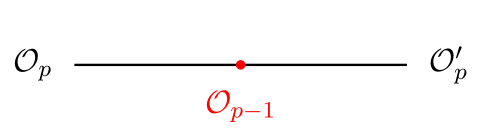
\includegraphics[scale=0.4]{figures/screening.png}
		\caption[Screening of operators]{Screening of operators.Taken from \cite{bhardwaj_lectures_2024}.}
	\end{figure}
	\noindent If $\mathcal{O}_p$ can be screened to the identity we say that it was completely screened. 
\end{definition}
\textbf{Screening implies in the same charges.} Note that if two operators $\mathcal{O}_p$ and $\mathcal{O}'_p$ are screened, we can deform the symmetry operator, say $U_g(S^{D-p-1})$, to measure the charge of either $\mathcal{O}_p$ or $\mathcal{O}'_p$. Since this deformation does not cross the regions where the operators are defined, the measured charges must be equal. The figure below represents this idea
\begin{figure}[H]
	\centering
	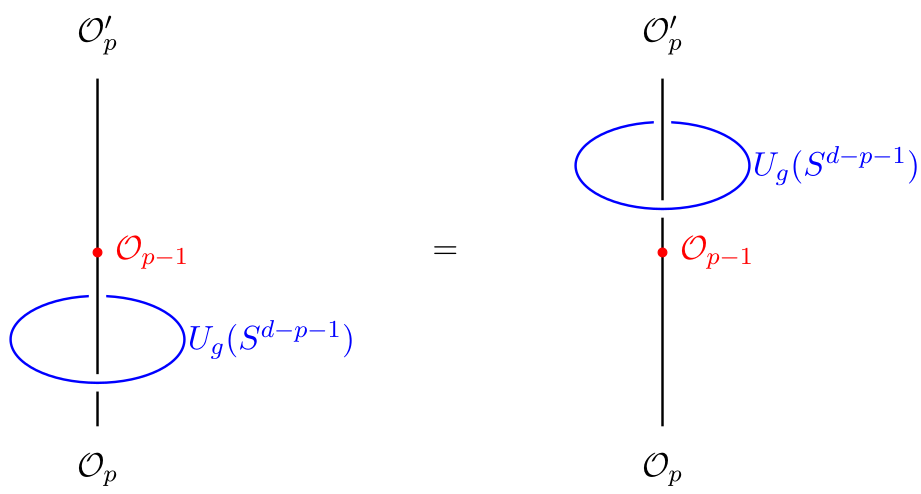
\includegraphics[scale=0.3]{figures/screening2.png}
	\caption[Link with two screened operators.]{Link with two screened operators. Taken from \cite{bhardwaj_lectures_2024}.}
\end{figure} 
\noindent If two operators carry different charges, they cannot be screened into another. 


As we have shown, the charges are given by phases. Each phase gives a different charges, that is 
\begin{equation}
	Q:G^{(p)}\to U(1).
\end{equation}
Therefore, the charge operators are elements of $\widehat{G}^{(p)}$. 
Thus, we may define an equivalence class of operators with the equivalence relation $\sim$ characterized by whether these operators can be screened into one another, 
\begin{equation*}
	\mathcal{O}_p'\sim \mathcal{O}_p.
\end{equation*}
We define the set $D_p$, where each element of this set is an equivalence class of screened operators. Therefore, there must exist $p$-form symmetries that distinguish different elements of $D_p$. The elements of $D_p$ are precisely the different charges that some operator might have, then 
\begin{equation*}
	\widehat{G}^{(p)}=D_p,
\end{equation*}
which implies
\begin{equation*}
	G^{(p)}=\widehat{D}_p.
\end{equation*}
Hence 
\begin{equation}
	Q(\mathcal{O}_p)=[\mathcal{O}_p]\in D_p.
\end{equation}
\subsubsection*{Example: Maxwell Theory in the presence of matter fields}
We have seen in Maxwell theory that we have a 1-form symmetry and a $(D-3)$-form symmetry\footnote{Actually, Maxwell theory is specifically in $D=4$, in which we have two 1-form symmetries. But for simplicity we just keep calling this way.}. But in order to have those symmetries, we evaluated the theory in the vacuum, that is 
\begin{equation*}
	d\star F=0.
\end{equation*}
The question that one can ask is: what if we add matter? We can understand the behavior using the concept of screening. 

We have seen that in the vacuum case, the symmetry group is $U(1)_e\times U(1)_m$. The Pontryagin dual is 
\begin{align*}
	&\widehat{G}^{(1)}=\mathbb{Z},\\
	&\widehat{G}^{(D-3)}=\mathbb{Z}.
\end{align*}
Therefore, 
\begin{align*}
	&D_1=\mathbb{Z},\\
	&D_{D-3}=\mathbb{Z}.
\end{align*}
Suppose now we add a matter field $\phi(x)$ with charge $N\in\mathbb{Z}$. We can use the operator $\phi(x)$ to screen the Wilson lines
\begin{figure}[H]
	\centering
	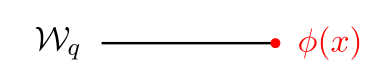
\includegraphics[scale=0.4]{figures/screening_wilson.png}
	\caption[Non-genuine operator.]{Non-genuine operator. Taken from \cite{bhardwaj_lectures_2024}.}
\end{figure}
\noindent We say then that $\phi(x)$ is a \textit{non-genuine} operator. 
\begin{definition}[Non-genuine operator]
	A non-genuine q-dimensional operator is an operator that is attached to a collection of $p>q$-dimensional operators. 
\end{definition}
We must introduce these non-genuine operators because $\phi(x)$ and $W_q(L)$ are not gauge invariant, since
\begin{equation}
	\phi(x)\to e^{iq\Lambda(x)}\phi(x)
\end{equation}
and 
\begin{equation}
	W_q(L)=\exp\left(2\pi iq\int_LA\right)\to\exp\left(2\pi iq\int_L A-\frac{d\Lambda}{2\pi}\right)=W_q\exp\left(-iq\int_{\partial L}\Lambda\right).
\end{equation}
Assuming that $\partial L=x$, 
\begin{equation}
	W_q'(L)=e^{-iq\Lambda(x)}W_q(L).
\end{equation}
Therefore the product $\phi(x)W_q(L)$ is gauge invariant. With this, we can screen several Wilson lines by adding powers of $\phi$
\begin{figure}[H]
	\centering
	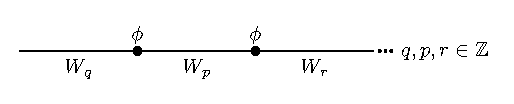
\includegraphics{figures/screening_wilson_n.pdf}
	\caption{Screening of multiple Wilson lines using powers of $\phi$.}
\end{figure}
Thus, the group of all unscreened operators will be given by the total number of Wilson lines minus the number of screened Wilson lines,
\begin{equation}
	D_1=\frac{\mathbb{Z}}{N\mathbb{Z}}\equiv\mathbb{Z}_N.
\end{equation}
Note that $N\mathbb{Z}$ counts the number of screened Wilson lines because, since they have the same charge, the charges add up N times. Taking the Pontryagin dual 
\begin{equation}
	\widehat{D}_1=\widehat{\mathbb{Z}}_N=\mathbb{Z}_N=G^{(1)}. 
\end{equation}
Then, we conclude that, adding a matter field with charge N breaks the gauge group $U(1)\to\mathbb{Z}_N$. The term ``break'' is not quite correct since gauge symmetries are not physical symmetries. The correct term that can be found in the literature is that the symmetry group is \textit{Higgsed-down} to $\mathbb{Z}_N$. Note that this does not happen with the $(D-3)$-form symmetry since this symmetry is associated with a codimension-2 operator that does not have a trivial link with the Wilson line. 
\subsubsection{BF Theory}
Now we can proceed and show how to obtain the BF theory starting from the usual Abelian Higgs model. The Lagrangian is 
\begin{equation}
	\L=|(\partial_\mu+iNA_\mu)\phi|^2-V(|\phi|)-\frac{1}{4}F_{\mu\nu}^2-NA_\mu j^{\mu},
\end{equation}
where the field $\phi$ has charge $N$. In the Higgs phase we get 
\begin{equation}\label{higgs phase lagrangian}
	\L = v^2(\partial_\mu\varphi+NA_\mu)^2-\frac{1}{4}F_{\mu\nu}^2-NA_\mu j^{\mu}.
\end{equation}
One could think on integrate out the field $\varphi$ to obtain an effective Lagrangian, but we cannot perform a straightfoward integration since  $\phi$ admit vortex solutions.
This implies that $\varphi$ has non-trivial winding. First, we need to split the phase $\varphi$ as
\begin{equation}\label{field split}
	\varphi=\tilde{\varphi}+\eta,
\end{equation}
where $\tilde{\varphi}$ provides information about the winding and the vortex positions and $\eta$ is a smooth function.
Then, we introduce the dual field $\xi_\mu$ with the Lagrangian
\begin{equation}
	\mathcal{L} = -\frac{1}{2v^2}\xi_\mu^2 + \xi_\mu(\partial^\mu\varphi-NA^\mu)-\frac{1}{4}F_{\mu\nu}^2-NA_\mu j^{\mu}.
\end{equation}
Note that computing the equations of motion for $\xi_\mu$ and substituing back into this Lagrangian lead us back to (\ref{higgs phase lagrangian}). Now we use (\ref{field split}), 
\begin{equation}
	\mathcal{L} = -\frac{1}{v^2}\xi_\mu^2 + \xi_\mu(\partial_\mu\tilde{\varphi}+\partial_\mu\eta - NA_\mu)-\frac{1}{4}F_{\mu\nu}^2-NA_\mu j^{\mu}.
\end{equation}
When we integrate over $\eta_\mu$ using a Gaussian integral  $\partial_\mu\xi^\mu=0$ then we may write
\begin{equation}
	\xi^{\mu}=\frac{iN}{2\pi}\epsilon^{\mu\nu\rho}\partial_\nu b_\rho,
\end{equation}
for some vector field $b_\rho$. The factor $iN/2\pi$ will be explained below. Then we get
\begin{equation}
	\begin{split}
		\mathcal{L} &= -\frac{1}{2v^2}\epsilon^{\mu\nu\rho}\epsilon_{\mu\alpha\beta}\partial_\nu b_\rho\partial_\alpha b_\beta + \frac{iN}{2\pi}\epsilon_{\mu\nu\rho}\partial^\nu b^{\rho}(\partial^\mu\tilde{\varphi}-NA^\mu) -\frac{1}{4}F_{\mu\nu}^2-NA_\mu j^{\mu} \\&
		= \frac{1}{2v^2}(f_{\mu\nu}^b)^2+ \frac{iN}{2\pi}\epsilon_{\mu\nu\rho}\partial^\nu b^{\rho}(\partial^\mu\tilde{\varphi}-NA^\mu) -\frac{1}{4}F_{\mu\nu}^2-NA_\mu j^{\mu},
	\end{split}
\end{equation}
where $f_{\mu\nu}^b = \partial_\mu b_\nu - \partial_\nu b_\mu$. Integrating the term $\epsilon_{\mu\nu\rho}\partial^\nu b^\rho\partial^\mu\tilde{\varphi}$ by parts we get 
\begin{equation}
	\mathcal{L} = \frac{1}{4\pi^2v^2}(f_{\mu\nu}^b)^2-\frac{iN}{2\pi}\epsilon_{\mu\nu\rho}b^\rho\partial^\nu\partial^\mu\tilde{\varphi} - \frac{iN^2}{2\pi}\epsilon_{\mu\nu\rho}\partial^\nu b^\rho A^\mu -\frac{1}{4}F_{\mu\nu}^2-NA_\mu j^{\mu}. 
\end{equation}
It looks like the second term is identically zero, but that is not true. The derivatives do not commute in consequence of the non-trivial winding of $\tilde{\varphi}$. Note that the quantity that couples with $b_0$ is $\frac{N}{2\pi}\epsilon_{ij}\partial_i\partial_j\tilde{\varphi}=\frac{N}{2\pi}\vec{\nabla}\times(\vec{\nabla}\tilde{\varphi})$. Integrating this in a region that contains the vortex leads to 
\begin{equation}
	\frac{N}{2\pi}	\int d^2x\;\vec{\nabla}\times(\vec{\nabla}\tilde{\varphi}) = \frac{N}{2\pi}\underbrace{\oint d\vec{x}\cdot \nabla\tilde{\varphi}}_{2\pi} = N. 
\end{equation}
This implies that this term is the density of vortices, that is, the zeroth component of some vortex current $\tilde{j}^\mu$, 
\begin{equation}
	\tilde{j}_\mu = \frac{N}{2\pi}\epsilon_{\mu\nu\rho}\partial_{\mu}\partial_{\nu}\tilde{\varphi},
\end{equation} 
where the factor $\frac{N}{2\pi}$ was only to ensure we get the total charge when integrated over all space. Then, we end up with the Lagrangian 
\begin{equation}
	\mathcal{L} = \frac{1}{2v^2}(f_{\mu\nu}^b)^2-\tilde{j}_\mu b^\mu -\frac{iN^2}{2\pi}\epsilon_{\mu\nu\rho}\partial^\nu b^\rho A^\mu - \frac{1}{4}F_{\mu\nu}^2-NA_\mu j^\mu. 
\end{equation}
Note from (\ref{higgs phase lagrangian}) that if we perform the gauge transformation 
\begin{equation}
	A_\mu \to A_\mu - \frac{1}{N}\partial_\mu\eta,
\end{equation}
at low energies, when $v^2\to\infty$, we have that 
\begin{equation}
	A_\mu \to -\frac{1}{N}a_\mu,
\end{equation}
where $a_\mu = \partial_\mu\tilde{\varphi}$. 
Hence, we get the BF Lagrangian 
\begin{equation}
	\mathcal{L} = \frac{1}{2v^2}(f_{\mu\nu}^b)^2- \frac{1}{4}(f_{\mu\nu}^a)^2- b^\mu\tilde{j}_\mu+a_\mu j^\mu +\frac{iN}{2\pi}\epsilon_{\mu\nu\rho}\partial^\nu b^\rho a^\mu . 
\end{equation}

To evaluate the higher-form symmetries in BF theory, we take the pure BF action in terms of differential forms,
\begin{equation}
	S_{BF}=\frac{iN}{2\pi}\int b\wedge da,
\end{equation}
The equations of motion for $b$ leads to 
\begin{equation}
	da=0\Rightarrow d\star(\star a)=0.
\end{equation}
Then, the conserved charge is 
\begin{equation}
	Q=\int_C a,
\end{equation}
where $C$ is a curve. If we instead write 
\begin{equation}
	S_{BF}=-\frac{iN}{2\pi}\int a\wedge db,
\end{equation}
and compute the equations of motion for $A$, we get 
\begin{equation}
	db=0,
\end{equation}
with the conserved current given by 
\begin{equation}
	Q=\int_{C'}b,
\end{equation}
where $C'$ is also a curve. The unitary operators are (with unit charge) 
\begin{align}
	&W_A(C)=e^{i\int a},\\
	&W_B(C')=e^{i\int b}.
\end{align}
Therefore, the conserved quantities of the 2+1 BF theory are the Wilson lines for the $a$ and $b$ fields. Note that this theory, just as Chern-Simons, is purely topological, i.e, it does not involve the metric. Now, the idea is the same as we did for Chern-Simons. From the Action we can compute the canonical momenta (using the gauge $a_0=b_0=0$),
\begin{equation}
	\begin{split}
		&\Pi_1^b=\Pi_2^b=0,\\
		&\Pi_1^a=\frac{\partial \mathcal{L}}{\partial \dot{a}_1}=-\frac{iN}{2\pi}b_2,\\
		&\Pi_2^a=\frac{\partial \mathcal{L}}{\partial \dot{
				a}_2}=\frac{iN}{2\pi}b_1.
	\end{split}
\end{equation}
And the commutation relations 
\begin{equation}
	\comm{a_i(x)}{\Pi_j^a(y)}=i\delta_{ij}\delta(x-y),
\end{equation}
leads to 
\begin{align}
	&\comm{a_1(x)}{b_2(y)}=-\frac{2\pi}{N}\delta(x-y),\label{comm a1b2}\\
	&\comm{a_2(x)}{b_1(y)}=\frac{2\pi}{N}\delta(x-y),\label{comm a2b1}\\
	&\comm{a_1(x)}{\Pi_2^a(y)}=\comm{a_2(x)}{\Pi_1^a(y)}=0.
\end{align}
This implies that,
\begin{equation}\label{degeneracy 1}
	W_1^aW_2^b=e^{-\frac{2\pi i}{N}}W_2^bW_1^a.
\end{equation}
On the other hand, since $W^A$ and $W^B$ are symmetries, it commute with the Hamiltonian. Therefore we have the same conclusion that we had for Chern-Simons. The energy  eigenstates are degenerate. It looks like the degeneracy is of order $N$, but we considered only the commutator (\ref{comm a1b2}). We need to consider the commutator (\ref{comm a2b1}) as well, 
\begin{equation}\label{degeneracy 2}
	W_2^aW_1^b=e^{-\frac{2\pi i}{N}}W_1^bW_2^a.
\end{equation}
Hence, we get a $N$-fold degeneracy from Eq.(\ref{degeneracy 1}) and a $N$-fold degeneracy from Eq.(\ref{degeneracy 2}), leading to a $N^2$-fold degeneracy. 


Recalling how we arrived at BF theory, we had to introduce a scalar field of charge $N$. As shown in the previous section, this breaks the symmetry group from $U(1)$ down to $\mathbb{Z}_N$. This implies that the gauge field $a$ has discrete gauge transformations, but what about the field $b$?

Note that if we start from the BF theory
\begin{equation}
	\mathcal{L} = \frac{iN}{2\pi}\epsilon_{\mu\nu\rho}\partial^{\mu}b^\nu a^\rho
\end{equation}
and add an auxiliary field $\hat{a}$ that enforces the constraint $f=da$, 
\begin{equation}
	\mathcal{L} = \frac{iN}{2\pi}\epsilon_{\mu\nu\rho}\partial^{\mu}b^\nu a^\rho + \frac{i}{2\pi}\partial_\mu\hat{a}_\nu f^{\mu\nu},
\end{equation}
we can rewrite the Lagrangian as 
\begin{equation}
	\mathcal{L} = -\frac{iN}{4\pi}\epsilon_{\mu\nu\rho} b^{\mu}f^{\nu\rho} - \frac{1}{4}(f_{\mu\nu})^2 + \frac{i}{2\pi}\partial_{\mu}\hat{a}_\nu f^{\mu\nu}. 
\end{equation}
Then, we integrate out $f_{\mu\nu}$. This will lead to 
\begin{equation}
	\mathcal{L} = \frac{iN}{2\pi}(\partial_\mu\hat{a}_\nu-N\epsilon_{\mu\nu\rho}b^\rho)^2. 
\end{equation}
But this Lagrangian has the same form as the Lagrangian on Eq.(\ref{higgs phase lagrangian}). Hence, by analogy, we can see the dual field $\hat{a}$ as a matter field which is charged under $b$. Therefore the BF theory is an example of a discrete gauge theory. 

\bibliography{refs.bib}
\bibliographystyle{ieeetr}
\end{document}
